\frametitle{Docking results of Mephenytoin}
\begin{columns}
	\begin{column}{0.6\linewidth}
		\begin{figure}
			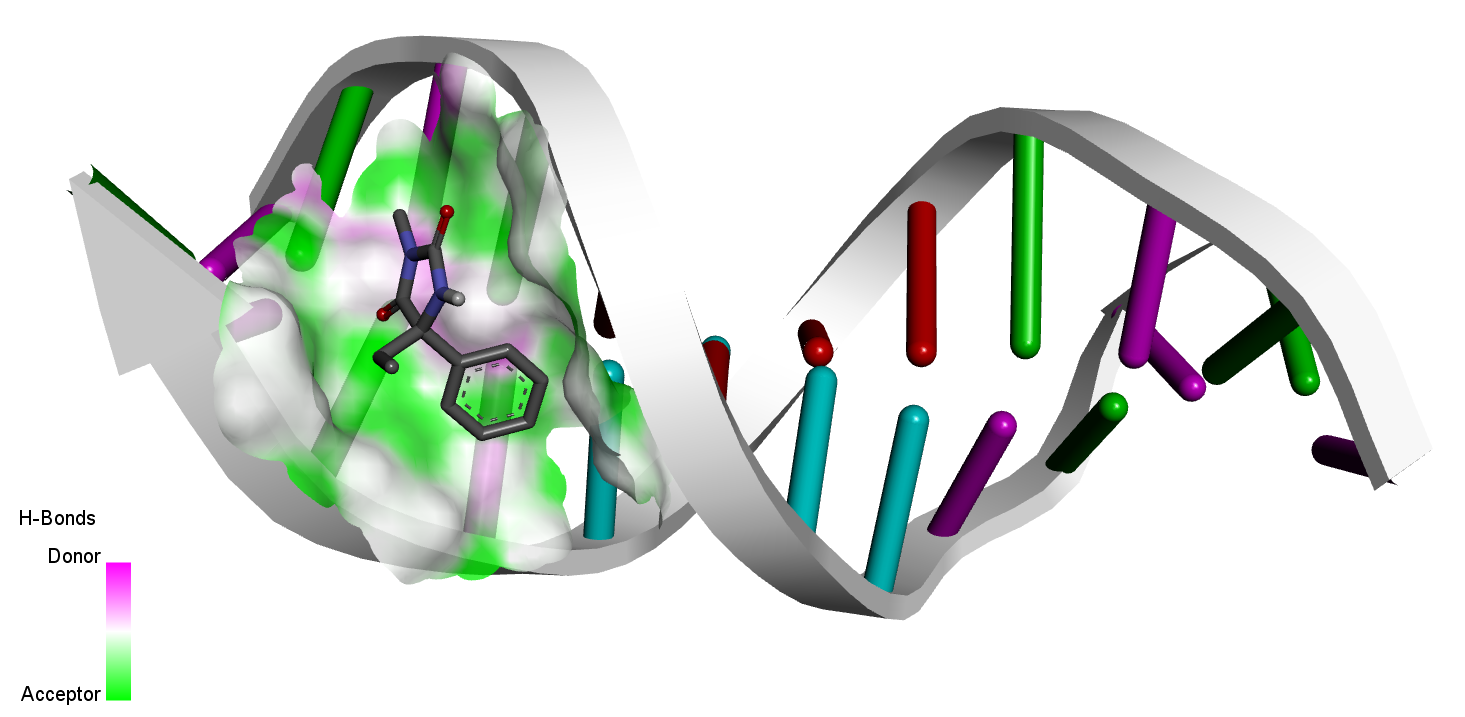
\includegraphics[width=\linewidth]{mepheytoin-donor-acceptor.png}
			\caption{\centering The donor-acceptor interaction \linebreak between Mephenytoin and B-DNA.}
			\label{fig:mph_donor_acceptor}
		\end{figure}
	\end{column}
	\begin{column}{0.45\linewidth}
		\centering
		\scriptsize
		\begin{table}
			\begin{tabular}{*{4}{c}}
				\hline\\[-1em]
				\multirow{2}{2em}{\centering\textbf{Mode}}&\multirow{2}{4em}{\centering\textbf{Affinity (kcal/mol)}}&\multicolumn{2}{c}{\centering\textbf{Distance from best mode}}\\
				\cline{3-4}
				&&\textbf{rmsd l.b.}&\textbf{rmsd u.b.}\\
				1&-6.0&0.000&0.000\\
				2&-6.0&0.225&1.217\\
				3&-5.9&2.588&4.660\\
				4&-5.6&1.942&2.857\\
				5&-5.4&1.453&1.985\\
				6&-5.3&2.002&4.710\\
				7&-5.2&1.916&5.436\\
				8&-5.1&2.079&4.524\\
				9&-5.0&2.357&3.786\\
				\hline
			\end{tabular}
			\caption{\centering The binding affinities and RMSD values between Mephenytoin and B-DNA.}
			\label{table:mph}
		\end{table}
	\end{column}
\end{columns}